\chapter{Amplificadores Realimentados}

\hspace{10pt}
Obtener en forma teórica la respuesta en frecuencia y la respuesta
al escalón del circuito de la figura \ref{lab1_1}.


\begin{figure}[h]
	\centering
	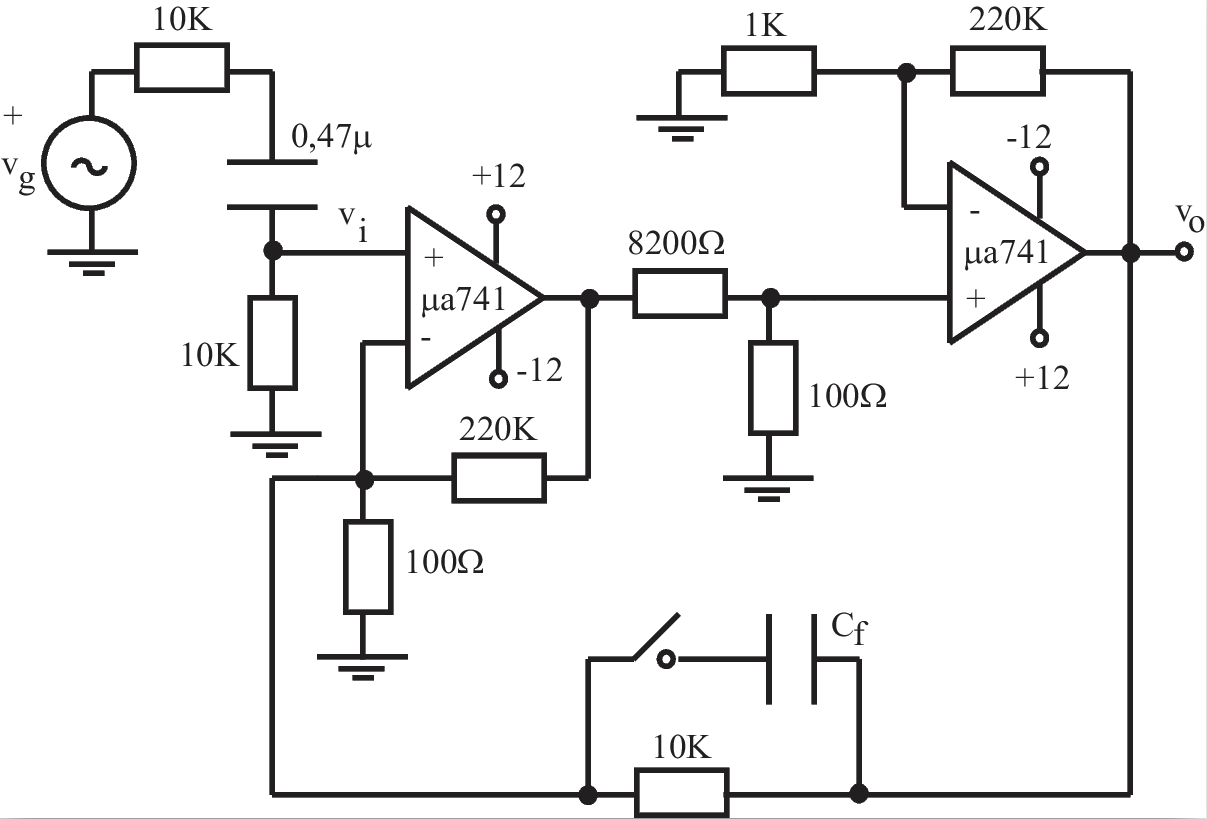
\includegraphics[width=0.8\linewidth]{figuras/lab1_1.png}\\
	\caption{}\label{lab1_1}
\end{figure}


Seguir los siguientes pasos:


\begin{enumerate}
	\item Utilizando un generador senoidal de frecuencia variable como entrada
	$v_g$ (usar $\sim 100 mV$ de amplitud de entrada), medir la magnitud
	de la ganancia $\frac{\displaystyle v_o}{\displaystyle v_i}$
	(utilizar las dos puntas de prueba de un osciloscopio) en función de
	la frecuencia. Comenzar en una frecuencia de 1 KHz , ir aumentando
	gradualmente la frecuencia de modo de obtener el valor de ganancia
	máximo, y la frecuencia a la que esto ocurre, luego seguir
	aumentando la frecuencia hasta encontrar la frecuencia de 0 dB. Con
	estos valores confeccionar una tabla y graficar en forma aproximada
	el diagrama de Bode de amplitud. La tabla y el Bode deben tener un
	``aspecto'' similar al de la figura \ref{lab1_2}.
	
	\item Utilizar un generador de onda cuadrada como entrada para evaluar la respuesta al escalón,
	con el osciloscopio medir los distintos parámetros de dicha respuesta, y con ellos calcular el Sobre Impulso porcentual
	($S.I.\% $) y estimar la ubicación de los polos del sistema realimentado. Utilice las siguientes expresiones, midiendo los parámetros mostrados en la figura \ref{lab1_3}
	
	\begin{eqnarray*}
		\nonumber
		SI \% &=& \frac{\displaystyle V_1}{\displaystyle V} 100 \\
		\nonumber
		\alpha [Hz] &=& \frac{\displaystyle 1}{\displaystyle 2 \pi T}\ln  \frac{\displaystyle V_1}{\displaystyle V_2}\\
		\nonumber
		\beta[Hz] &=& \frac{\displaystyle 1}{\displaystyle T}
	\end{eqnarray*}
	
	\item Compensar el circuito mediante el agregado de $C_f$, ¿Qué valor de
	$C_f$ elegiría y con qué criterio lo haría?
	
	\item Realizar las simulaciones de la respuesta en frecuencia y
	la respuesta al escalón del circuito propuesto, variando en forma
	paramétrica $C_f$ desde 0 hasta el doble del valor diseñado en 3.
	Obtener también por simulación el margen de fase para cada caso de
	$C_f$. Comparar los resultados con los datos obtenidos por medición
	y en forma teórica.
	
	\item Confeccionar un informe escrito completo de la
	Práctica de Laboratorio, incluyendo mediciones, simulaciones y
	cálculos teóricos.
\end{enumerate}

\begin{figure}[h]
	\centering
	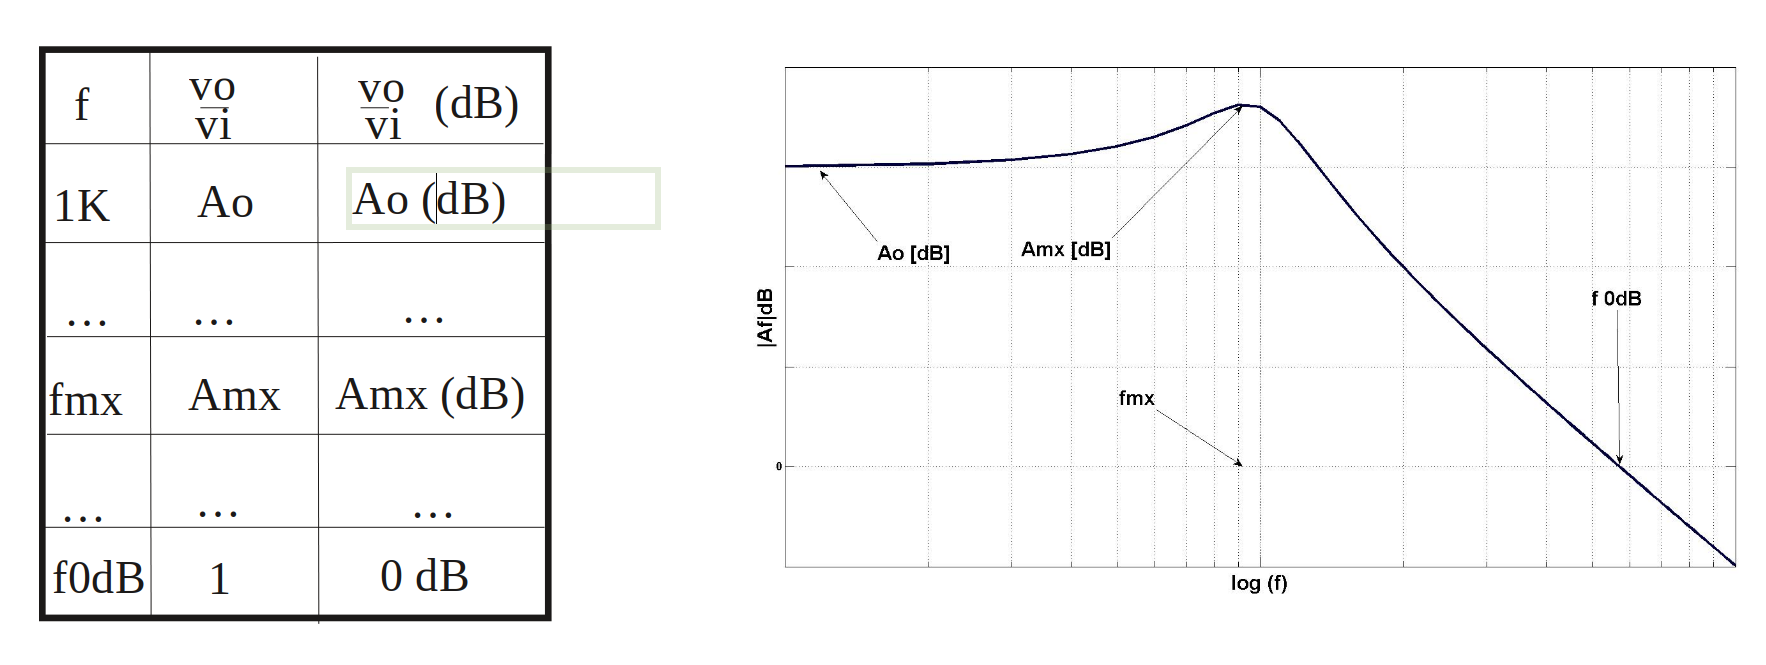
\includegraphics[width=0.8\linewidth]{figuras/lab1_2.png}\\
	\caption{}\label{lab1_2}
\end{figure}

\begin{figure}[h]
	\centering
	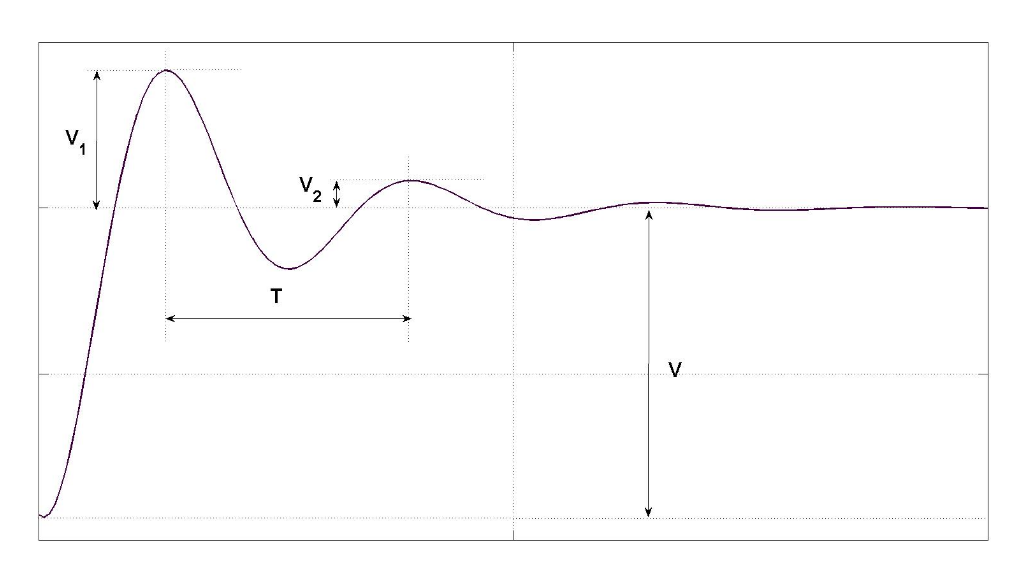
\includegraphics[width=0.8\linewidth]{figuras/lab1_3.png}\\
	\caption{}\label{lab1_3}
\end{figure}
